%--------------------------------------%
%----- 2_Versuchsvorbereitung.tex -----%
%--------------------------------------%
%--------------------------------------%
%
%
%
%
% Bitte denkt daran, eure Autorenschaft namentlich zu kennzeichnen! Das gilt für jeden (Unter-)Abschnitt, den ihr bearbeitet habt.
%
In diesem Experiment soll die Resonanz auf einem Resonanzkreis der RLC-Reihenschaltung untersucht werden. Der erste Schritt besteht darin, die theoretisch erwarteten Kurven von Strom und Gesamtimpedanz als Funktion der Eingangsfrequenz zu bestimmen. Im zweiten Schritt ist die Schaltung einzurichten und die Frequenzcharakteristik durch Messung zu bestimmen. Im dritten Schritt sollte die Schaltung in LTspice eingerichtet und simuliert werden, um idealisierte Profile der Frequenzverlaufe zu erhalten. Schließlich werden die theoretischen, gemessenen und die aus der Simulation erhaltenen Ergebnisse beschrieben, verglichen und interpretiert.
\begin{flushright}
  \textit{\autorA}
\end{flushright}
%
%
%
\subsection{Herableitung Resonanzfrequenz}
Die Resonazfrequenz ist die Frequenz die der großte Amplitudenantwort hat
Wenn wir die Resonanzfrequenz $f$ finden wollen, können wir z.B die Maxima von Bodeplot ablesen. Mathematisch finden wir die übertragungsfunktion von entweder $\underline{U}_\qty{R,C,L}$ und finden ihre Betragmaxima.

Beispielweise ist die Übertragungsfunktion \[\frac{U_R}{U_{ein}}=\frac{Z_R}{Z_R+Z_L+Z_C}=\frac{R}{R+sL+\frac{1}{sC}}\]
Es ist am großten wenn $R+sL+\frac{1}{sC}$ am kleinsten wird, bzw $Z_{ges}=Z_{min}.$
Wir ersetzen $s=\imag \omega.$
Und leiten wir $\omega$ ab. Setzen wir es gleich 0 an.
\[\imag\qty(L+\frac{1}{C \omega^2})=0\>\omega^2=-\frac{1}{C L}\>\omega_0=\mp \frac{1}{\sqrt{CL}}\]
Da $\omega = 2 \pi f$ dann ist unsere \[f_0=\frac{1}{2 \pi \sqrt{C L}}.\]

Die Zeigerdiagram an die Resonanzfrequenz bei unsere Schaltung würde so aussehen. Bei $f=f_0$
\begin{figure}[H]
  \centering
  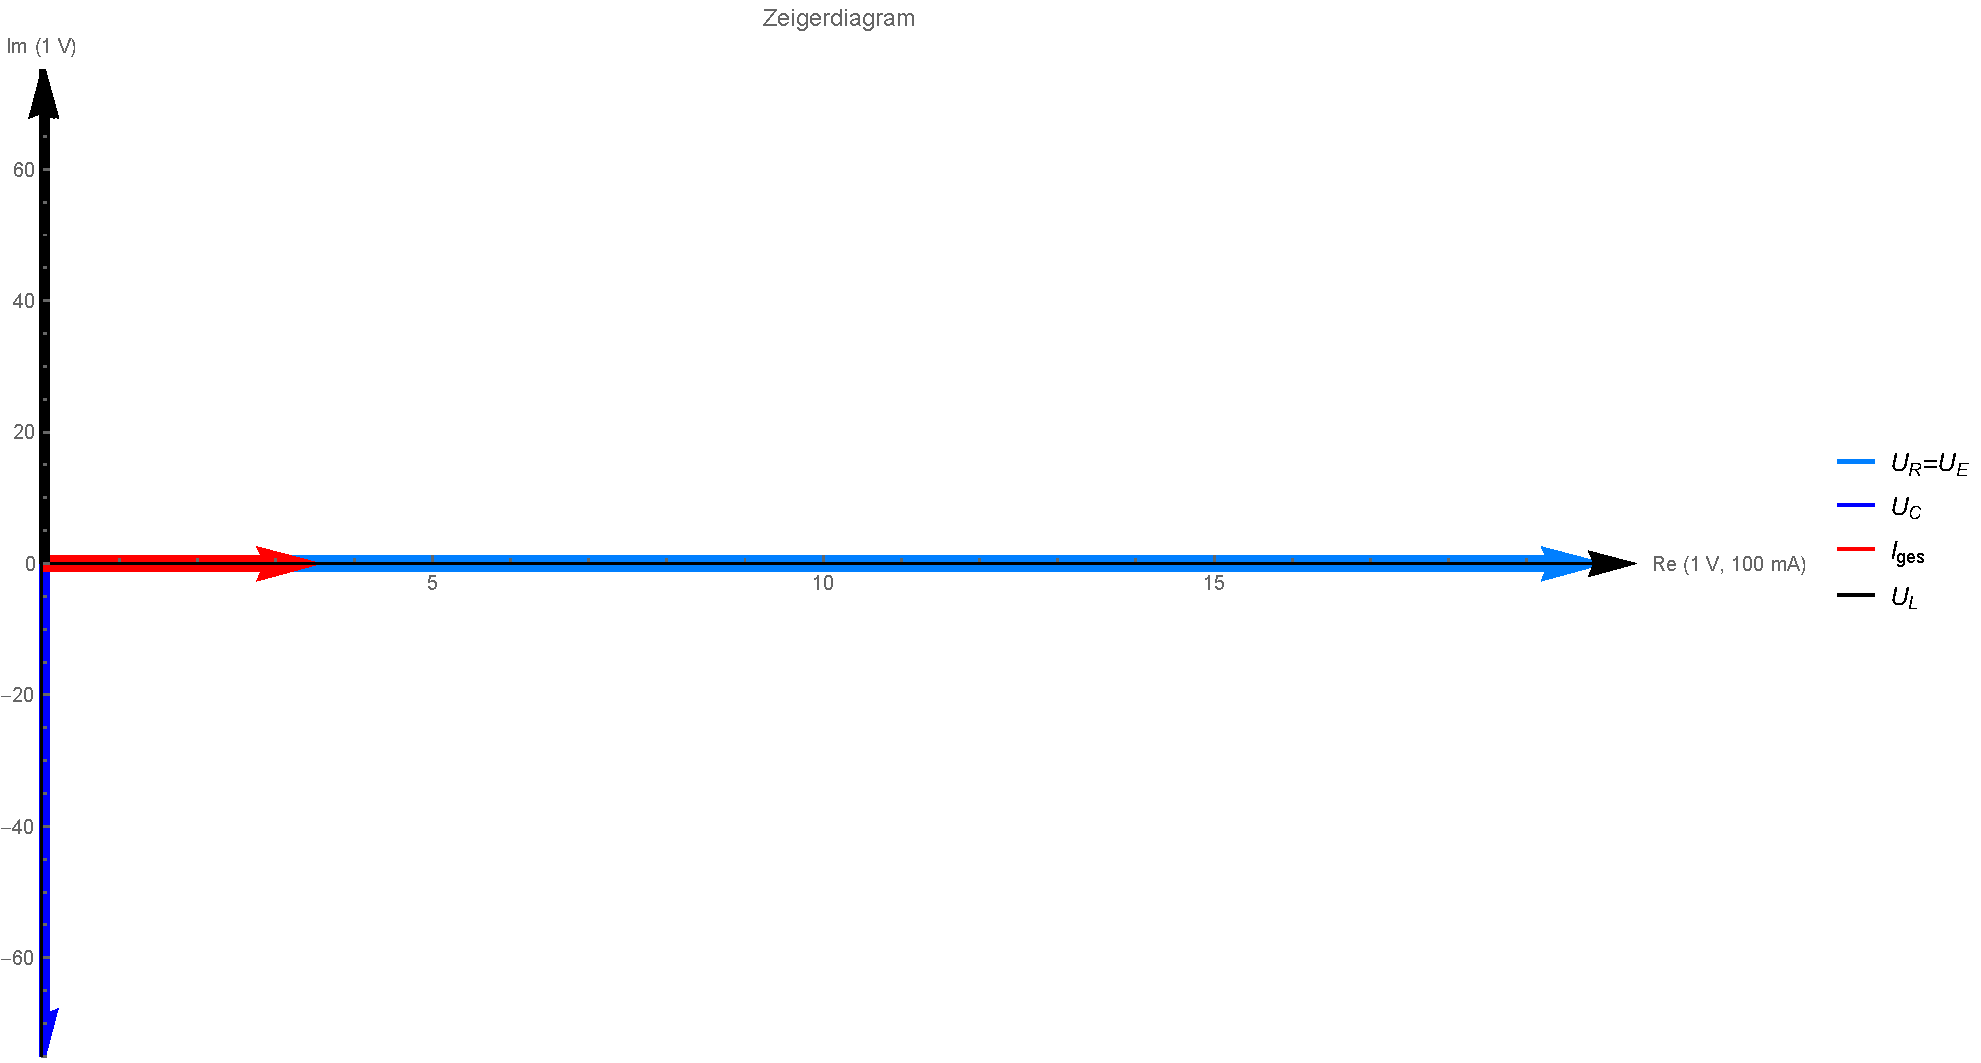
\includegraphics[width=0.9\linewidth]{src/elnw3.pdf}
  \caption{Zeigerdiagram}
  \label{fig:3_Sim_Spannungsquelle}
\end{figure}
%
%\lipsum[3]
%
%
%
% Bitte denkt daran, eure Autorenschaft namentlich zu kennzeichnen! Das gilt für jeden (Unter-)Abschnitt, den ihr bearbeitet habt.
%
%\begin{flushright}
%  \textit{\autorA}
%\end{flushright}
%
%
%
%\subsection{Bspw. zur Berechnung theoretischer Messgrößenverläufe}
%
%\lipsum[5]
%
%
%
% Bitte denkt daran, eure Autorenschaft namentlich zu kennzeichnen! Das gilt für jeden (Unter-)Abschnitt, den ihr bearbeitet habt.
%
%\begin{flushright}
%  \textit{\autorA}
%\end{flushright}
%
%
%
